\ifTombow\addtocontents{toc}{\protect\newpage}\fi
\hyperchapter{ch34}{rvalueリファレンス}{rvalueリファレンス}
\index{rvalueりふあれんす@\texttt{rvalue}リファレンス}

\hypersection{ch3401}{概要}

いままで使っているリファレンスは、正式には\texttt{lvalue}リファレンスという名前がついている。これは\texttt{lvalue}へのリファレンスという意味だ。\texttt{lvalue}へのリファレンスがあるからには、\texttt{lvalue}ではないリファレンスがあるということだ。C++には\texttt{rvalue}へのリファレンスがある。これを\texttt{rvalue}リファレンスという。

この章で説明する内容はとても難しい。完全に理解するためには、何度も読み直す必要があるだろう。

\hypersection{ch3402}{rvalueリファレンスの宣言}
\index{rvalueりふあれんす@\texttt{rvalue}リファレンス!せんげん@宣言}

\texttt{T}型への\texttt{lvalue}型リファレンス型は\texttt{T \&}\,と書く。

\begin{lstlisting}[language={C++}]
T & lvalue_reference = ... ;
\end{lstlisting}

\texttt{T}型への\texttt{rvalue}リファレンス型は\texttt{T \&\&}\,と書く。
\index{T \&\&@\texttt{T \&\&}}\index{rvalueりふあれんす@\texttt{rvalue}リファレンス!T \&\&@\texttt{T \&\&}}

\begin{lstlisting}[language={C++}]
T && rvalue_reference = ... ;
\end{lstlisting}

\texttt{lvalue}リファレンスは\texttt{lvalue}で初期化する。\texttt{rvalue}リファレンスは\texttt{rvalue}で初期化する。

\texttt{lvalue}とは名前付きのオブジェクトや戻り値の型としての\texttt{lvalue}リファレンスのことだ。

\ifTombow\pagebreak\fi
\begin{lstlisting}[language={C++}]
int object { } ;
int & f() { return object ; }

int main()
{
    // lvalueリファレンス
    int & a = object ;
    int & b = f() ;
}
\end{lstlisting}

ここで、式\texttt{object}や式\texttt{f()}を評価した結果は\texttt{lvalue}だ。

\texttt{rvalue}とは、名前なしのオブジェクトや計算結果の一時オブジェクト、戻り値の型としての\texttt{rvalue}リファレンスのことだ。

\begin{lstlisting}[language={C++}]
int && g() { return 0 ; }
int h() { return 0 ; }

int main()
{
    // rvalueリファレンス
    int && a = 0 ;
    int && b = 1 + 1 ;
    int && c = g() ;
    int && d = h() ;
}
\end{lstlisting}

ここで、式\texttt{0}、式\texttt{1 + 1}、式\texttt{g()}を評価した結果は\texttt{rvalue}だ。

\texttt{rvalue}リファレンスを\texttt{lvalue}で初期化することはできない。

\begin{lstlisting}[language={C++}]
int object { } ;
int & f() { return object ; }

int main()
{
    // すべてエラー
    int && a = object ;
    int && b = f() ;
}
\end{lstlisting}

\texttt{lvalue}リファレンスを\texttt{rvalue}で初期化することはできない。

\ifTombow\pagebreak\fi
\begin{lstlisting}[language={C++}]
int && g() { return 0 ; }
int h() { return 0 ; }

int main()
{
    // すべてエラー
    int & a = 0 ;
    int & b = 1 + 1 ;
    int & c = g() ;
    int & d = h() ;
}
\end{lstlisting}

リファレンスを初期化することを、リファレンスはリファレンス先を束縛\index{そくばく@束縛}するという。\texttt{lvalue}リファレンスは\texttt{lvalue}を束縛する。\texttt{rvalue}リファレンスは\texttt{rvalue}を束縛する。

ただし、\texttt{const}な\texttt{lvalue}リファレンスは\texttt{rvalue}を束縛することができる。

\begin{lstlisting}[language={C++}]
int && g() { return 0 ; }

int main()
{
    // OK、constなlvalueリファレンス
    const int & a = 0 ;
    const int & b = 1 + 1 ;
    const int & c = g() ;
}
\end{lstlisting}

\texttt{rvalue}リファレンス自体は\texttt{lvalue}だ。なぜならば\texttt{rvalue}リファレンスはオブジェクトに名前を付けて束縛するからだ。

\begin{lstlisting}[language={C++}]
int main()
{
    // rvalueリファレンス
    int && a = 0 ;
    // OK、rvalueリファレンスaはlvalue
    int & b = a ;
    // エラー、 rvalueリファレンスaはrvalueではない
    int && b = a ;
}
\end{lstlisting}

\clearpage
\hypersection{ch3403}{値カテゴリー}
\index{あたいかてごり@値カテゴリー}

\texttt{lvalue}と\texttt{rvalue}とは何か。もともと\texttt{lvalue}\index{lvalue@\texttt{lvalue}}とは左辺値(left--hand value)\index{さへんち@左辺値}、\texttt{rvalue}\index{rvalue@\texttt{rvalue}}とは右辺値(right--hand value)\index{うへんち@右辺値}という語源を持っている。これはまだC言語すらなかったはるか昔から存在する用語で、代入式の左辺に書くことができる値を\texttt{lvalue}、右辺に書くことができる値を\texttt{rvalue}と読んでいたことに由来する。

\begin{lstlisting}[language={C++}]
lvalue = rvalue ;
\end{lstlisting}

例えば、\texttt{int}型の変数\texttt{x}は代入式の左辺に書くことができるから\texttt{lvalue}、整数リテラル\texttt{0}は右辺に書くことができるから\texttt{rvalue}といった具合だ。

\begin{lstlisting}[language={C++}]
int x ;
x = 0 ;
\end{lstlisting}

C++では\texttt{lvalue}と\texttt{rvalue}をこのような意味では使っていない。

\texttt{lvalue}と\texttt{rvalue}を理解するには、値カテゴリーを理解しなければならない。

\begin{enumerate}
\def\labelenumi{\arabic{enumi}.}
\item
  式(expression)とは\texttt{glvalue}か\texttt{rvalue}である。
\item
  \texttt{glvalue}とは\texttt{lvalue}か\texttt{xvalue}である。
\item
  \texttt{rvalue}とは\texttt{prvalue}か\texttt{xvalue}である。
\end{enumerate}

この関係を図示すると以下のようになる。

\begin{figure}[htbp]
  \centering
  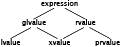
\includegraphics[scale=1.0]{fig/fig37-01.eps}
  \label{fig:37-01}
\end{figure}

\hypersubsection{ch340301}{lvalue}
\index{lvalue@\texttt{lvalue}}

\texttt{lvalue}はすでに説明したとおり名前付きのオブジェクトのことだ。

\begin{lstlisting}[language={C++}]
// lvalue
int object ;
int & ref = object ;
\end{lstlisting}

通常使うほとんどのオブジェクトは\texttt{lvalue}になる。

\hypersubsection{ch340302}{prvalue}
\index{prvalue@\texttt{prvalue}}

\texttt{prvalue}は純粋な\texttt{rvalue}(pure rvalue)のことだ。つまり、名前なしのオブジェクトや計算結果の一時オブジェクトのことだ。

\begin{lstlisting}[language={C++}]
int f() { return 0 ; }

// prvalue
0 ;
1 + 1 ;
f() ;
\end{lstlisting}

ほとんどの\texttt{prvalue}は式を評価するときに自動的に生成され、自動的に破棄されるので、あまり意識することはない。

関数の戻り値の型がリファレンスではない場合、一時オブジェクトが生成される。

\begin{lstlisting}[language={C++}]
struct X { } ;
X f() ;
\end{lstlisting}

演算子も関数の一種なので、
\begin{lstlisting}[language={C++}]
auto result = x + y + z ;
\end{lstlisting}
のような式がある場合、まず\texttt{x + y}が評価され、その結果が一時オブジェクトとして返される。その一時オブジェクトを仮に\texttt{temp}とすると、\texttt{temp + z}が評価され、また一時オブジェクトが生成され、変数\texttt{result}に代入される。

式文全体を評価し終わったあとに、一時オブジェクトは自動的に破棄される。

一時オブジェクトは自動的に生成され、自動的に破棄される。ここがとても重要な点だ。これは次の章で説明するムーブセマンティクスに関わってくる。

\hypersubsection{ch340303}{xvalue}
\index{xvalue@\texttt{xvalue}}

\texttt{xvalue}とは寿命が尽きかけている\texttt{lvalue}(eXpiring lvalue)のことだ。\texttt{xvalue}は\texttt{lvalue}や\texttt{prvalue}から変換することで発生する。

\texttt{xvalue}となる値は以下のような場合だ。

\vskip 1.0zw
\noindent
\(\bullet\) \textsf{戻り値の型がオブジェクトの型への\texttt{rvalue}リファレンスである関数の呼び出しの結果}

\begin{lstlisting}[language={C++}]
int && f() { return 0 ; }

int main()
{
    // xvalue
    int && r = f() ;
}
\end{lstlisting}

%\vskip 1.0zw
\ifTombow\pagebreak\fi
\noindent
\(\bullet\) \textsf{オブジェクトの型への\texttt{rvalue}リファレンスへのキャスト}

\begin{lstlisting}[language={C++}]
int main()
{
    int object{} ;
    // xvalue
    int && r = static_cast<int &&>(object) ;
}
\end{lstlisting}

\vskip 1.0zw
\noindent
\(\bullet\) \textsf{\texttt{xvalue}配列\index{xvalueはいれつ@\texttt{xvalue}配列}への添字操作}

\begin{lstlisting}[language={C++}]
int main()
{
    int a[3] = {1,2,3} ;
    int && r = static_cast<int (&&)[3]>(a)[0] ;
}
\end{lstlisting}

\texttt{xvalue}配列というのは配列のオブジェクトを配列への\texttt{rvalue}リファレンス型にキャストすると得られる。\texttt{xvalue}配列への添字操作の結果は\texttt{xvalue}だ。

\vskip 1.0zw
\noindent
\(\bullet\) \textsf{\texttt{xvalue}なクラスのオブジェクトへのリファレンスではない非\texttt{static}データメンバーへのアクセス}

\begin{lstlisting}[language={C++}]
struct X { int data_member ; } ;

int main()
{
    X x{} ;
    int && r = static_cast<X &&>(x).data_member ;
}
\end{lstlisting}

\vskip 1.0zw
\noindent
\(\bullet\) \textsf{式\,\texttt{.*}\,で最初のオペランドが\texttt{xvalue}で次のオペランドがデータメンバーへのポインターの場合}

\begin{lstlisting}[language={C++}]
struct X { int data_member ; } ;

int main()
{
    X x{} ;
    int && r = static_cast<X &&>(x).*&X::data_member ;
}
\end{lstlisting}

これも配列と似ていて、\texttt{xvalue}のクラスオブジェクトに対するメンバーへのポインター経由でのメンバーの参照結果は\texttt{xvalue}になるということだ。

%\vskip 1.0zw
\ifTombow\pagebreak\fi
重要なのは最初の2つだ。残りは覚える必要はない。重要なのは、\texttt{xvalue}とは、\texttt{lvalue}か\texttt{prvalue}から変換した結果発生するものだ。

\hypersubsection{ch340304}{rvalue}
\index{rvalue@\texttt{rvalue}}

\texttt{prvalue}と\texttt{xvalue}を合わせて、\texttt{rvalue}という。\texttt{rvalue}リファレンスというのは、\texttt{rvalue}でしか初期化できない。\texttt{rvalue}というのは\texttt{prvalue}か\texttt{xvalue}のどちらかだ。

\texttt{lvalue}は\texttt{xvalue}に変換できるので、結果として\texttt{rvalue}に変換できることになる。

\begin{lstlisting}[language={C++}]
int main()
{
    // lvalueなオブジェクト
    int lvalue { } ;

    // OK、lvalueリファレンスはlvalueで初期化できる
    int & l_ref = lvalue ;

    // OK、rvalueリファレンスはrvalueで初期化できる
    // rvalueリファレンスにキャストした結果はrvalue
    int && r_ref = static_cast<int &&>(lvalue) ;
}
\end{lstlisting}

\texttt{lvalue}はそのままでは\texttt{rvalue}ではないが、\texttt{xvalue}に変換すれば\texttt{rvalue}になる。

\texttt{prvalue}はもともと\texttt{rvalue}である。

この性質は次の章で説明するムーブセマンティクスで利用する。

\hypersubsection{ch340305}{glvalue}
\index{glvalue@\texttt{glvalue}}

\texttt{glvalue}は一般的な\texttt{lvalue}(generalized lvalue)という意味だ。\texttt{glvalue}とは、\texttt{lvalue}か\texttt{xvalue}のことだ。

\texttt{lvalue}から変換した\texttt{xvalue}はもともと\texttt{lvalue}だったのだから、\texttt{glvalue}となるのも自然だ。\texttt{xvalue}に変換した\texttt{prvalue}は\texttt{glvalue}になれる。

この性質はムーブセマンティクスで利用する。

\clearpage
\hypersection{ch3404}{rvalueリファレンスのライブラリ}

\hypersubsection{ch340401}{std::move}
\index{move@\texttt{move}}

\texttt{std::move(e)}は値\texttt{e}を\texttt{xvalue}にするための標準ライブラリだ。\texttt{std::move(e)}は値\texttt{e}の型\texttt{T}への\texttt{rvalue}リファレンス型にキャストしてくれるので、\texttt{xvalue}になる。そして\texttt{xvalue}は\texttt{rvalue}だ。

\begin{lstlisting}[language={C++}]
int main()
{
    int lvalue { } ;
    int && r = std::move(lvalue) ;
}
\end{lstlisting}

これは以下のように書いたものと同じようになる。

\begin{lstlisting}[language={C++}]
int main()
{
    int lvalue { } ;
    int && r = static_cast<int &&>(lvalue) ;
}
\end{lstlisting}

\hypersubsection{ch340402}{std::moveの実装}
\index{move@\texttt{move}!じつそう@実装}

\texttt{std:move(e)}の実装は少し難しい。根本的には、式\texttt{e}のリファレンスではない型\texttt{T}に対して、\texttt{static\_cast<T \&\&>(e)}をしているだけだ。

すると以下のような実装だろうか。

\begin{lstlisting}[language={C++}]
template < typename T >
T && move( T & t ) noexcept
{
    return static_cast<T &&>(t) ;
}
\end{lstlisting}

この実装は\texttt{lvalue}を\texttt{xvalue}に変換することはできるが、\texttt{rvalue}(\texttt{prvalue}と\texttt{xvalue})を\texttt{xvalue}に変換することはできない。

\begin{lstlisting}[language={C++}]
int main()
{
    // エラー、 prvalueを変換できない
    int && r1 = move(0) ;

    int lvalue { } ;
    // エラー、 xvalueをxvalueに変換できない
    int && r2 = move(move(lvalue)) ;
}
\end{lstlisting}

\texttt{rvalue}は\texttt{rvalue}リファレンスで受け取れるので、\texttt{lvalue}リファレンスを関数の引数として受け取る\texttt{move}のほかに、\texttt{rvalue}リファレンスを関数の引数として受け取る\texttt{move}を書くとよい。

すると以下のように書けるだろうか。

\begin{lstlisting}[language={C++}]
// lvalueリファレンス
template < typename T >
T && move( T & t ) noexcept
{
    return static_cast<T &&>(t) ;
}

// rvalueリファレンス
template < typename T >
T && move( T && t ) noexcept
{
    return static_cast<T &&>(t) ;
}
\end{lstlisting}

しかしこれでは関数の本体の中身がまったく同じ関数が2つできてしまう。もっと複雑な関数を書くときにこのようなコードの重複があると、ソースコードの修正が難しくなる。せっかくテンプレートを使っているのにこれでは意味がない。

\hypersubsection{ch340403}{フォワーディングリファレンス}
\index{ふおわでいんぐりふあれんす@フォワーディングリファレンス}

C++のテンプレートはコードの重複を省くためにある。そのため、C++ではテンプレートパラメーターへの\texttt{rvalue}リファレンスを関数の仮引数として取る場合を、フォワーディングリファレンス(forwarding reference)として、特別に\texttt{lvalue}でも\texttt{rvalue}でも受け取れるようにしている。

\begin{lstlisting}[language={C++}]
// T &&はフォワーディングリファレンス
template < typename T >
void f( T && t ) ;
\end{lstlisting}

このような関数テンプレートの仮引数\texttt{t}に実引数として\texttt{rvalue}を渡すと、\texttt{T}は\texttt{rvalue}の型となり、結果として\texttt{t}の型は\texttt{T \&\&}\,になる。

\begin{lstlisting}[language={C++}]
// Tはint
f(0) ;
\end{lstlisting}

もし実引数として型\texttt{U}の\texttt{lvalue}を渡すと、テンプレートパラメーター\texttt{T}が\texttt{U \&}\,となる。そして、テンプレートパラメーター\texttt{T}に対するリファレンス宣言子(\texttt{\&}, \texttt{\&\&})は単に無視される。

\begin{lstlisting}[language={C++}]
int lvalue{} ;
// Tはint &
// T &&はint &
f(lvalue) ;
\end{lstlisting}

ここで、関数テンプレート\texttt{f}のテンプレートパラメーター\texttt{T}は\texttt{int \&}\,となる。この\texttt{T}にリファレンス宣言子を\texttt{T \&}\,や\texttt{T \&\&}\,のように使っても、単に無視されて、\texttt{T \&}\,となる。

\begin{lstlisting}[language={C++}]
template < typename T >
void f( T && t )
{
    using A = T & ;
    using B = T && ; 
}

int main()
{
    // prvalue
    f(0) ;
    int lvalue{} ;
    // lvalue
    f(lvalue) ;
}
\end{lstlisting}

\texttt{f(0)}は\texttt{prvalue}を渡している。この場合、\texttt{T}の型は\texttt{int}となる。\texttt{A}は\texttt{int \&}、\texttt{B}は\texttt{int \&\&}\,となる。

\texttt{f(lvalue)}は\texttt{lvalue}を渡している。この場合、\texttt{T}の型は\texttt{int \&}\,となる。この場合の\texttt{T}に\,\texttt{\&}\,や\,\texttt{\&\&}\,を付けても無視される。なので、\texttt{A}, \texttt{B}の型はどちらも\texttt{int \&}\,になる。

したがって、以下のように書くと\texttt{move}は\texttt{lvalue}も\texttt{rvalue}も受け取ることができる。

\begin{lstlisting}[language={C++}]
// lvalueもrvalueも受け取ることができるmove
template < typename T >
T && move( T && t ) noexcept
{
    return static_cast<T &&>(t) ;
}
\end{lstlisting}

ただし、この実装にはまだ問題がある。この\texttt{move}に\texttt{lvalue}を渡した場合、\texttt{lvalue}の型を\texttt{U}とすると、テンプレートパラメーター\texttt{T}は\texttt{U \&}\,になる。

\begin{lstlisting}[language={C++}]
U lvalue{} ;
// TはU &
move( lvalue ) ;
\end{lstlisting}

テンプレートパラメーター名\texttt{T}がリファレンスのとき、\texttt{T}にリファレンス宣言子\,\texttt{\&\&}\,を付けても単に無視されることを考えると、上の\texttt{move}に\texttt{int \&}\,型の\texttt{lvalue}が実引数として渡されたときは、以下のように書いたものと等しくなる。

\begin{lstlisting}[language={C++}]
int & move( int & t ) noexcept
{
    return static_cast<int &>(t) ;
}
\end{lstlisting}

\texttt{move(e)}は\texttt{e}が\texttt{lvalue}であれ\texttt{rvalue}であれ、\texttt{xvalue}にする関数だ。そのためには、\texttt{rvalue}リファレンスにキャストしなければならない。テンプレートではフォーワーディングリファレンスという例外的な仕組みによって\texttt{lvalue}も\texttt{rvalue}も\texttt{T \&\&}\,で受け取れるが、\texttt{lvalue}を受け取ったときには\texttt{T \&\&}\,が\texttt{lvalue}リファレンスになってしまうのでは、\texttt{xvalue}にキャストできない。

この問題は別のライブラリによって解決できる。

\hypersubsection{ch340404}{std::remove\texttt{\_}reference\texttt{\_}t}
\index{remove\_reference\_t@\texttt{remove\_reference\_t}}

\texttt{std::remove\_reference\_t<T>}\,は\texttt{T}型からリファレンス型を除去してくれるライブラリだ。

\begin{lstlisting}[language={C++}]
int main()
{
    // int
    using A = std::remove_reference_t<int> ;
    // int
    using B = std::remove_reference_t<int &> ;
    // int
    using C = std::remove_reference_t<int &&> ;
}
\end{lstlisting}

ということは、これとリファレンス宣言子を組み合わせると、どのような型がテンプレート実引数に渡されても\texttt{rvalue}リファレンスにできる。

\begin{lstlisting}[language={C++}]
template < typename T >
void f()
{
    using RT = std::remove_reference_t<T> && ;
}
\end{lstlisting}

\texttt{add\_pointer\_t/remove\_pointer\_t}があるように、\texttt{remove\_reference\_t}にも対となるリファレンスを追加するライブラリが存在する。ただしリファレンスには\texttt{lvalue}リファレンスと\texttt{rvalue}リファレンスがあるので、それぞれ\texttt{std::add\_lvalue\_reference\_t<T>}\,\index{add\_lvalue\_reference\_t@\texttt{add\_lvalue\_reference\_t}}、\texttt{std::add\_rvalue\_reference\_t<T>}\,\index{add\_rvalue\_reference\_t@\texttt{add\_rvalue\_reference\_t}}となっている。

\ifTombow\pagebreak\fi
\begin{lstlisting}[language={C++}]
int main()
{
    // int &
    using A = std::add_lvalue_reference_t<int> ;
    // int &&
    using B = std::add_rvalue_reference_t<int> ;
}
\end{lstlisting}

\hypersubsection{ch340405}{std::moveの正しい実装}
\index{move@\texttt{move}}

\texttt{std::remove\_reference\_t<T>}\,を使うと、\texttt{move}は以下のように書ける。

\begin{lstlisting}[language={C++}]
template < typename T >
std::remove_reference_t<T> && move( T && t ) noexcept
{
    return static_cast< std::remove_reference_t<T> && >(t) ;
}
\end{lstlisting}

\hypersubsection{ch340406}{std::forward}
\index{forward@\texttt{forward}}

テンプレートパラメーターに\texttt{rvalue}リファレンス宣言子を使うと\texttt{lvalue}も\texttt{rvalue}も受け取れる。

\begin{lstlisting}[language={C++}]
template < typename T >
void f( T && t ) { }

int main()
{
    int lvalue{} ;
    f(lvalue) ;
    f(0) ;
}
\end{lstlisting}

この関数\texttt{f}から別の関数\texttt{g}に値を渡したい場合を考えよう。

\begin{lstlisting}[language={C++}]
template < typename T >
void g( T && t ) { }

template < typename T >
void f( T && t )
{
    g(t) ;
}
\end{lstlisting}

このとき、関数\texttt{f}に渡されたものが\texttt{lvalue}でも\texttt{rvalue}でも、関数\texttt{g}に渡される値は\texttt{lvalue}になってしまう。

なぜならば、名前付きの\texttt{rvalue}リファレンスに束縛されたオブジェクトは\texttt{lvalue}だからだ。

\begin{lstlisting}[language={C++}]
int main()
{
    // 名前付きのrvalueリファレンス
    int && rvalue_ref = 0 ;
    // これはlvalue
    int & lvalue_ref = rvalue_ref ;
}
\end{lstlisting}

なので、\texttt{g(t)}の\texttt{t}は\texttt{lvalue}となる。

ここで\texttt{rvalue}を渡すのは簡単だ。\texttt{std::move}を使えばいい。

\begin{lstlisting}[language={C++}]
template < typename T >
void f( T && t )
{
    g( std::move(t) ) ;
}
\end{lstlisting}

ただし、これは\texttt{t}が\texttt{lvalue}のときも問答無用で\texttt{xvalue}にしてしまう。

\texttt{t}が\texttt{lvalue}ならば\texttt{lvalue}として、\texttt{rvalue}ならば\texttt{xvalue}として、渡された値カテゴリーのまま別の関数に渡したい場合、\texttt{std::forward<T>(t)}が使える。

\begin{lstlisting}[language={C++}]
template < typename T >
void f( T && t )
{
    g( std::forward<T>(t) ) ;
}
\end{lstlisting}

\texttt{std::forward<T>(t)}の\texttt{T}にはテンプレートパラメーター名を書く。こうすると、\texttt{t}が\texttt{lvalue}ならば\texttt{lvalue}リファレンス、\texttt{rvalue}ならば\texttt{rvalue}リファレンスが戻り値として返される。

\texttt{std::forward}の実装は以下のとおりだ。

\begin{lstlisting}[language={C++}]
template<class T>
constexpr 
T &&
forward(remove_reference_t<T>& t) noexcept
{ return static_cast<T&&>(t) ; }

(@\ifTombow\pagebreak\fi@)
template<class T>
constexpr 
T &&
forward(remove_reference_t<T>&& t) noexcept
{ return static_cast<T&&>(t) ; }
\end{lstlisting}

もし\texttt{std::forward<T>(t)}に\texttt{lvalue}が渡された場合、上の\texttt{forward}が呼ばれる。その場合、\texttt{T}は\texttt{lvalue}リファレンスになっているはずなので\texttt{rvalue}リファレンス宣言子は無視され、\texttt{lvalue}リファレンスが戻り値の型になる。

\texttt{rvalue}が渡された場合、\texttt{rvalue}リファレンスが戻り値の型になる。
